\bgroup{}

\chapter{Methods}\label{cha:methods}
This chapter explains the methods needed for accomplishing the motives described in \cref{sec:motive}. Establishing a sound analysis strategy, finding similar sounds, and predicting user categorization are some of the necessary components for the proposed system. Each section clarifies the choice of a particular procedure over comparable ones. As the author has no prior knowledge of the subject, the decision process progressed mostly through research and planning, with a great deal of trial and error involved.

\section{Audio analysis}\label{sec:audio_analysis}
One objective required for the suggested system described in \cref{sec:motive} is the possibility to handle digital audio files in a programming environment. In order to interpret sounds programmatically, some form of conversion needs to take place, processing sound files to data applicable for a computer. There are different strategies for generating metadata from sounds, but the approach favored in this thesis is an interpretation with timbral characteristics.

Generally, timbre is a word describing perceptual attributes of a sound, excluding pitch and loudness, spatial and musicological descriptors, as well as higher-level cognitive properties~\cite[7]{rep:d5.1}. In more general terms, timbre is what enables humans – and probably other species – to distinguish one sounding object from another, even though the pitch, loudness, and duration remain constant. For example, if a violin and a piano play the same note at equal volume for a fixed period, it is still possible to differentiate the two instruments by their sound quality alone.

Many published methods are available that represent the timbre of a sound in different data-oriented ways, often in the form of an object containing metadata. The model used in~\cite{unpub:the_timbral_model} illustrates a way of analyzing sounds using analog equipment. As most work transpires digitally today, this process has advanced accordingly;~\cite{rep:constructing_high-level_perceptual_audio_descriptors_for_textural_sounds} describes a computerized assembled counterpart. Numerous tools and libraries built on these concepts are available for analyzing and describing sounds. For instance,~\cite{rep:mirtoolbox} presents a tool containing functions dedicated to the extraction of musical features from audio files, and~\cite{rep:sra} exhibits a web-based tool that performs spectral and roughness analysis on user-submitted sound files. A notable instance of an open-source library is \emph{Essentia}~\cite{essentia, rep:essentia} developed by \gls{mtg}, competent in audio analysis and audio-based music information retrieval to a high degree. Another popular library is \emph{LibROSA}~\cite{librosa, rep:librosa}, used for audio and music signal analysis. These systems are capable of much more than just producing timbral metadata, as they can track the beat of a song, work out the tempo, along with other features.

All of the described methods use one or more algorithms, either established or custom-made ones, to manage sounds and produce an output. Some projects keep the algorithms secret while others, like with \emph{Essentia}, have them available to the public. Defining various adjective-based descriptions that function as dividers and designating each sound with a numeric value for every descriptor is another typical pattern among the systems. Combining words like `roughness', `sharpness', or similar with a number is something found in many of the methods for deriving timbral values. The studies in~\cite{rep:words_that_describe_timbre_a_study_of_auditory_perception_through_language} and~\cite[20]{rep:d5.1} are examples of studies that provide comprehensive lists of words describing timbre.

The selected method for analyzing audio in this thesis is the \emph{AudioCommons Timbral Models} package~\cite{timbral_models} developed by the \gls{iosr} for the AudioCommons project funded by the European Union~\cite{audiocommons}. It is part of the \emph{Audio Commons Audio Extractor}, which \emph{Freesound}, for instance, has chosen to integrate into their service~\cite{ac-audio-extractor, freesound:integration}. Interestingly enough, the implemented package is dependant on the previously mentioned \emph{Essentia} and \emph{LibROSA} libraries for some of the calculations, but only provide a fraction of the features that they have~\cite[4]{rep:d5.2}\cite[5]{rep:d5.6}.

The timbral model package by \gls{iosr} can predict eight distinctive timbral characteristics from audio files of multiple formats, using a separate model for each characteristic. These eight models are all regression-based models, except for the classification model used to predict reverb qualities. This project omits the reverb model as it deviates from the other models' output and obstructs the sound similarity estimation method (see \cref{sec:sound_similarity_estimation}).

One of the seven remaining used models produces a \emph{hardness} value. The attack time, attack gradient, and spectral centroid of attack for a sound serve as parameters for a linear regression model, which generates said timbral characteristic. The model responsible for \emph{depth} works by analyzing the spectral centroid, the energy proportion, and potentially the limit of lower frequencies of input audio. A representation of \emph{brightness} models on a sound's spectral centroid variant and a spectral energy ratio of high frequencies, while \emph{roughness} models the interaction of similar amplitude and frequency peaks within the frequency spectrum. The three remaining timbral values, \emph{warmth}, \emph{sharpness}, and \emph{boominess}, are all implementations on previous models, which the associated papers describe and reference, but without any in-depth information.~\cite{rep:d5.2, rep:d5.6}

The seven resolved characteristics produced by the timbral model conclusively portray a sound timbrally in a metadata format. This procedure means that every analyzed sound receives seven corresponding attributes represented numeric values, ranging from 0 to 100. \Cref{fig:example-sound} shows an audio graph of an example sound, and \cref{tab:example-sound} shows the output of the same sound processed by the package.
\begin{figure}[ht]
    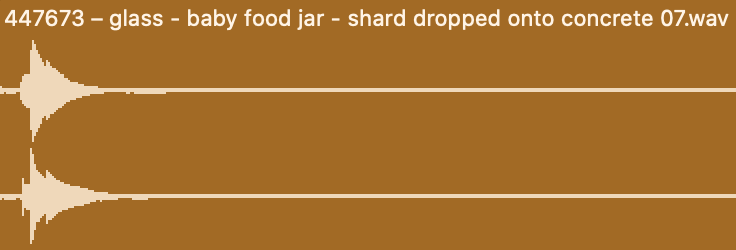
\includegraphics[width=\textwidth]{figures/methods/example-sound}
    \caption{Audio graph of an example sound.}\label{fig:example-sound}
\end{figure}
\begin{table}[ht]
    \caption{Predicted timbral values for the same example sound.}\label{tab:example-sound}
    \begin{tabular*}{\textwidth}{@{\extracolsep{\fill}}*{7}{r}}
        \toprule
        \emph{hardness} & \emph{depth} & \emph{brightness} & \emph{roughness} & \emph{warmth} & \emph{sharpness} & \emph{boominess} \\
        67.71 & 3.41 & 88.3 & 54 & 31.16 & 100 & 5.07 \\
        \bottomrule
    \end{tabular*}
\end{table}

The specified package is relatively straightforward to use, due to it being rather concentrated with only a few available scripts, which is one of the reasons for the author choosing to incorporate it into the developed system. Furthermore, the created set of timbral attributes seems to be of high-quality and covers a broad timbral spectrum. These aspects make it well suited as a building block for constructing prototypes, in which category the developed application falls, sequentially making it the chosen method for audio analysis in this thesis.

\section{Sound similarity estimation}\label{sec:sound_similarity_estimation}
The goals in \cref{sec:motive} oblige a strategy for understanding a user's definition of similar sounds. Different people may have a distinct threshold when segregating sounds depending on their perception. A sound engineer could classify two closely resembled audio tracks as separate sounds, while a more inexperienced listener puts them in the same category. There are no wrongs or rights, as it is only a matter of taste and preference. By using the predicted timbral attributes in \cref{sec:audio_analysis} as a foundation, it is possible to conceptualize a strategy that materializes into a system that can distinguish sounds the same way as the current user.

Since the seven characteristics described in \cref{sec:audio_analysis} represent sounds in the proposed solution of this thesis, the similarity of two sounds is consequently the difference between their predicted timbral values. Two sounds which merely vary with 50 units of \emph{hardness}, say if one sounds has a \emph{hardness} value of 25 and the other of 75, are equally dissimilar in portrayed timbre as if the difference was with 50 units of \emph{depth}. This formula builds on the axiom that all of the seven calculated timbral values are of equal significance. The difference sums of all timbral values between two sounds, like the \emph{hardness} difference of 50 in the previous example, collectively make up the distance between the sounds. Even though all characteristics have equal influence, the tolerance of when two similar sounds split into separate sounds could alter among the attributes. This definition means that a user might perceive sounds differing with a value of 25 \emph{hardness} as separate groups or classes, while only a difference of 15 \emph{depth} achieves the same effect; one could say the user is more sensitive to \emph{depth} changes. The suggested solution considers this with the support of multiple dimensions when searching for similar sounds, effectively meaning that each value corresponds to a point in a seven-dimensional coordinate system.
\begin{figure}[ht]
    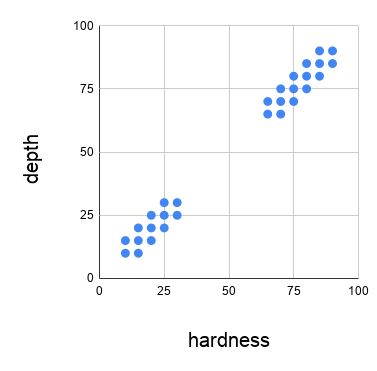
\includegraphics[width=0.495\textwidth]{figures/methods/chart-a}
    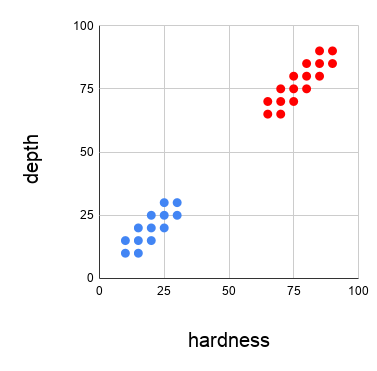
\includegraphics[width=0.495\textwidth]{figures/methods/chart-b}
    \caption[Example case were two users have categorized sounds differently.]{Example case were two users have categorized sounds differently. The {\color{blue}blue} color signifies once group and the {\color{red}red} another.}\label{fig:methods/charts}
\end{figure}

When comparing sounds as audio or timbrally calculated values, there could be more deciding factors that affect a user's decision process when perceiving sounds as equal or not. Alongside differences within the same timbral characteristic, cross-characteristic discrepancies could also affect a user's judgment. In order to illustrate this scenario, the following examples will consider only \emph{hardness}, \emph{depth}, and \emph{brightness}, or three dimensions. If two sounds have the same predicted values for \emph{hardness} and \emph{depth}, say 20 \emph{hardness} and 30 \emph{depth}, but different values for \emph{brightness}, e.g., 85 versus 90, a user could still want to categorize them independently. Even though two sets of the same timbral values are identical and the remaining two only differ with a modest distance of 5, the cross-distance of \emph{hardness}–\emph{brightness} and \emph{depth}–\emph{brightness} also contrasts when comparing the example sounds. This variance from one characteristic to another could affect how a user segregates sounds.

In contrast, a user could perhaps say two sounds still belong to a single group even when all the distances between the same timbral characteristics are relatively large. This situation could perchance happen when the ratios are constant, like if the values for one sound were 20 for every defined attribute and 30 for the other sound. These kinds of variations are right to consider, as audio perception and sound segregation are quite abstract and dynamic, depending on the circumstances.

\section{Machine learning}
Part of the aimed for requirements outlined in \cref{sec:motive} demands a component or subsystem intelligent enough to mimic and adapt to different definitions of sound similarity. The threshold variance among users when segregating sounds is what the desired component should try to learn as precisely as possible. The discussed theories in \cref{sec:sound_similarity_estimation} set a foundation for such a subsystem, which this section expands upon and substantiates using \gls{ml}.

\Acrlong{ml} is the act of programming a computer so that it learns from data without explicit instructions~\cite[26]{book:hands-on_machine_learning_with_scikit-learn_&_tensorflow}. In other words, the concept of \acrlong{ml} is to let the algorithms define and output the rules of a problem when given the data and the answers as input~\cite[28]{book:deep_learning_with_python}. Many fields of technology make use of \gls{ml} today to accomplish complex tasks. Speech recognition, spam filtering, and customizing web experiences are some areas that utilize \gls{ml} extensively~\cite[13]{book:hands-on_machine_learning_with_scikit-learn_&_tensorflow}. As each problem is unique with its idiosyncrasies, no single algorithm can handle every task, often referred to as the `No-Free-Lunch theorems' originating in~\cite[12]{rep:the_lack_of_a_priori_distinctions_between_learning_algorithms}. Therefore, it is first necessary to define the problem itself and all its challenges and quirks to know what style of \gls{ml} best fits the task at hand.

The goal of the asserted subsystem is to categorize sounds based on similarity into the same groups as a specific person would, without regulation or influence from other users. With this intention specified, the problem falls into the category of classification-based problems. The idea builds on the motive that each user's perception is unique enough that neglecting the element of a unified definition for sound similarity based on shared assumptions is tolerable~\cite[2]{rep:psychoacoustically_informed_spectrography_and_timbre}. As identical classifications of sounds among different persons could be quite common, this hypothesis is probably not entirely true. However, it is a generalization made in this thesis in order to achieve a functional system.

The subsystem should ergo initially operate without any presumed instructions, which also means it lacks directions on the concluding sum and division of classes. Evaluation for the component's accuracy comes from the users themselves when they interact with the proposed system planned in \cref{sec:motive}. This valuation transpires when the user verifies categorizations designated by the \gls{ml} algorithms in the developed program. With the adjustments, the number of correct classifications grows, and the subsystem receives more and more information and clues on how to segregate sounds according to the user's sound similarity definition. The continuous feedback from the user should improve the component accordingly. Finally, the size of the data collection of sounds to interpret can change, as the user can add more data to the developed application at any time, which the \gls{ml} procedure should take into consideration.

In \gls{ml} terms, these specifications signify that data collection and data preparation occur progressively and that all data is \emph{unlabeled}, i.e., unprocessed, in the beginning. More samples are converted to \emph{labeled} data as the user interacts with the system; in the end, when the user has verified every sample, all data is \emph{labeled}. When the user includes new \emph{unlabeled} data, it should undergo the same process until it is fully \emph{labeled}. A single static \gls{ml} algorithm is most likely insufficient, as the solution needs to improve gradually.

A dominant challenge of the described task is that it at least partially fits all the four major types of \gls{ml} currently established~\cite[30]{book:hands-on_machine_learning_with_scikit-learn_&_tensorflow}:

\begin{itemize}
    \item Supervised learning uses \emph{labeled} data as a training set to discover the mapping between a set of inputs and outputs~\cite[30]{book:hands-on_machine_learning_with_scikit-learn_&_tensorflow}. A typical task solved with supervised learning is classification, which suits the problem at hand. A hindrance is that no \emph{labeled} data is available, at least initially.
    \item Unsupervised learning tries to find usable patterns hidden within data without instructions, even when the input data is convoluted~\cite[32]{book:hands-on_machine_learning_with_scikit-learn_&_tensorflow}. These qualities make it suitable for the described task as \emph{unlabeled} data is present at practically all stages of the suggested system.
    \item Semi-supervised is a mix of supervised and unsupervised learning. This combination means that semi-supervised algorithms function with \emph{unlabeled} data, but require \emph{labeled} data for training, although in a smaller scale than supervised algorithms~\cite[35]{book:hands-on_machine_learning_with_scikit-learn_&_tensorflow}. Since \emph{labeled} data is unavailable at many times, as described earlier, the semi-supervised style has the same obstruction as the supervised type.
    \item Reinforcement learning deviates substantially from the other approaches, as it learns by itself using a positive and negative feedback system, an observer called `agent', and a strategy, or `policy', for scoring the most rewards over time~\cite[35]{book:hands-on_machine_learning_with_scikit-learn_&_tensorflow}. This method falls short as the end classification distribution is impossible to predict in advance, and due to the lack of scores to give the algorithms.
\end{itemize}

There are no doubt multiple algorithms and sequences of algorithms that manage to complete the outlined task. A combination of one or more unsupervised algorithms with some supervised or semi-supervised ones could probably work. One challenging bit, in that case, would be the interaction between the styles and understand which outputs to use in what scenarios. Reinforcement learning could also work if there were ways to construct the self-learning system that the algorithms demand.

The method that the author chose to implement uses two unsupervised learning algorithms: \emph{Mean shift} and \emph{K-means clustering}. The first creates a starting point for categorizing sounds based on similarity, and the other adjusts the estimation for every user interaction to better simulate the user's perception. The implemented application relies heavily on \emph{clustering}, or the act of detecting groups of elements with similar features, as it is the core concept for finding related sounds. \Cref{sec:sound_similarity} in the following chapter explains the two algorithms in more detail, how they synergy with each other, and how the proposed system uses them in a programming context.

\egroup{}